%*****************************************
\chapter{Mixed Methods}\label{ch14:mixed}
%*****************************************
%TODO Status: First draft

\section{Introduction}

There are, broadly speaking, two ways to approach a research project: quantitative and qualitative. Quantitative projects gather numeric data and analyze those data with statistical tools. Qualitative projects gather non-numeric data and analyze those data with non-mathematical tools. It is possible, though, to combine both types of analysis in a single research project, a process known as ``mixed methods.'' This chapter first reviews both quantitative and qualitative methods and then considers the process used to combine those methods.\footnote{This chapter is an expansion of information first presented in Chapter \ref{06:data}. Readers may want to review that material to help clarify concepts presented here.}

\section{Quantitative Analysis}
%TODO Bhattacherjee p 128

Numeric data collected in a research project can be analyzed quantitatively using statistical tools in two different ways. 

\begin{itemize}
	\item Descriptive analysis refers to statistically describing, aggregating, and presenting the constructs of interest or associations between these constructs. 

	\item Inferential analysis refers to the statistical testing of hypotheses (theory testing). 

\end{itemize}

Most quantitative data analysis is conducted using software programs such as R and the labs that accompany this text are designed to introduce that important software.

\subsection{Quantitative Analysis: Descriptive}
%TODO Bhattacherjee p 128
\subsubsection{Univariate Analysis}

Univariate analysis, or analysis of a single variable, refers to a set of statistical techniques that can describe the general properties of one variable. Univariate statistics include: (1) frequency distribution, (2) central tendency, and (3) dispersion. The frequency distribution of a variable is a summary of the frequency that individual values are found in a variable. For instance, it is easy to measure how often customers in a grocery store purchase types of products, like ``produce,'' ``dairy,'' and ``meat.'' If the number (or percentage) of observations within each category are counted and displayed in a table it would be called a \textit{frequency distribution}, as seen in Table \ref{14:tab01}. A frequency distribution can also be depicted in the form of a bar chart, as shown in Figure \ref{14:fig01}, with the horizontal axis representing number of purchases in each category and the vertical axis representing the categories.

\begin{table}[H]
	\centering
	\begin{tabulary}{\linewidth}{LR}
		\hline
		Item & Number \\ 
		\hline
		Produce & 374 \\ 
		Dairy & 291 \\ 
		Meat & 187 \\ 
		\hline
	\end{tabulary} 
	\caption{Frequency Table}
	\label{14:tab01}
\end{table}

\vspace{.15in}

\begin{figure}[H]
	\centering
	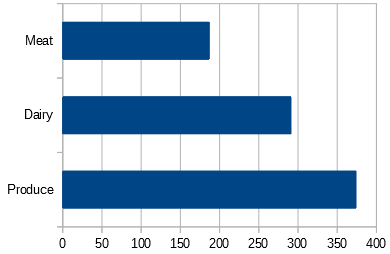
\includegraphics[width=\maxwidth{.95\linewidth}]{gfx/14-BarChart}
	\caption{Bar Chart}
	\label{14:fig01}
\end{figure}

With very large samples where observations are independent and random, the frequency distribution resembles a normal distribution, which looks like a bell-shaped curve when plotted. Figure \ref{14:fig02} shows the distribution of scores for the Scholastic Aptitude Test (\textit{SAT}) where most observations are clustered toward the center of the range with fewer observations toward the extremes. 

\begin{figure}[H]
	\centering
	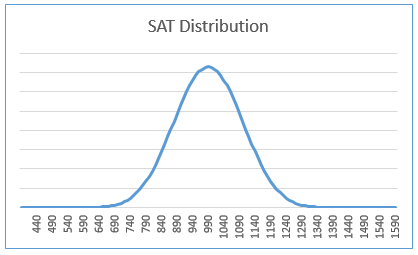
\includegraphics[width=\maxwidth{.95\linewidth}]{gfx/14-NormDist}
	\caption{Normal Distribution}
	\label{14:fig02}
\end{figure}

Central tendency is an estimate of the center of a distribution of values. There are three major estimates of central tendency: mean, median, and mode. The arithmetic mean (often simply called the ``mean'') is the simple average of all values in a given distribution. Consider a set of eight test scores: $ 15 $, $ 22 $, $ 21 $, $ 18 $, $ 36 $, $ 15 $, $ 25 $, $ 15 $. The arithmetic mean of these values is ($ 15 + 20 + 21 + 20 + 36 + 15 + 25 + 15)/8 = 20.875 $.

The median, is the middle value in a distribution. This is computed by ordering all values and selecting the one in the middle. In case there are two middle values (if there is an even number of values in a distribution), the median is the average of the two middle values. In the example test scores from the previous paragraph, the sorted values are: $ 15 , 15 , 15 , 18 , 22 , 21, 25, 36 $. The two middle values are $ 18 $ and $ 22 $ so the median is $ (18 + 22)/2 = 20 $. 

The mode is the most frequently occurring value in a distribution of values. Mode is normally only used for categorical data rather than numeric. For example, if an item on a survey asked whether respondents rented, leased, or owned their office building it would not make sense to try to find an ``average'' for those values, instead the most common response would be reported as the mode. 

Dispersion refers to the way values are spread around the central tendency, for example, how tightly or how widely are the values clustered around the mean. Two common measures of dispersion are the range and standard deviation. 

The range is the difference between the highest and lowest values in a distribution. The range in the test scores above is $ 36 - 15 = 21 $. The range is particularly sensitive to the presence of outliers, which makes its use problematic. For instance, if the highest value in the above distribution was $ 85 $ and the other vales remained the same, the range would be $ 85 - 15 = 70 $. 

Standard deviation corrects for outliers by calculating each value's distance from the mean. While that is a relatively complex calculation, all statistics software is able to easily find the standard deviation. In a normal distribution, 68\% of the observations lie within one standard deviation of the mean, 95\% within two standard deviations, and 99.7\% within three standard deviations.

\subsubsection{Bivariate Analysis}

Bivariate analysis examines how two variables are related to each other. The most common bivariate statistic is a correlation, which is a number between $ -1.00 $ and $ +1.00 $ denoting the strength and direction of the relationship between two variables. As an example, consider a data set that contains selected specifications found in the 1974 \textit{Motor Trend} magazine for 32 automobiles (1973–74 models)\footnote{The Motor Trend data was originally published in a report by Henderson and Vellerman in \textit{Biometrics}\cite{henderson1981building}.}. The first few items in that data set are shown in Table \ref{14:tab02}.

\begin{table}[H]
	\centering
	\begin{tabulary}{\linewidth}{LCCCCCC}
		\hline
		Name           & mpg    & cyl & disp  & hp    & wt      & qsec  \\ 
		\hline
		Mazda RX4      & $21.0$ & $6$ & $160$ & $110$ & $2.620$ & $16.46$ \\ 
		Datsun 710     & $22.8$ & $4$ & $108$ & $93$  & $2.320$ & $18.61$ \\ 
		Hornet 4 Drive & $21.4$ & $6$ & $258$ & $110$ & $3.215$ & $19.44$ \\ 
		Valiant        & $18.1$ & $6$ & $225$ & $105$ & $2.460$ & $20.22$ \\ 
		\hline
	\end{tabulary} 
	\caption{Sample of Motor Trend Car Data}
	\label{14:tab02}
\end{table}

Two of the variables in this data set are ``disp'' (engine displacement) and ``qsec'' (quarter-mile time, in seconds). It would be normal to expect that the greater the engine displacement (that is, the larger the engine) then the faster the automobile would finish a quarter-mile track. It turns out that the correlation between displacement and quarter-mile time is $ -0.43 $. The negative sign indicates that the relationship is negative, that is, as the displacement increases the time decreases. The magnitude of the correlation, though, indicates that this is not a particularly strong relationship, so a lot of small engines can finish the quarter-mile track as quickly as larger engines. A researcher would want to know why and one of the first confounding factors to consider would be the weight of the automobile. Are automobiles with larger engines also heavier, and, thus, slower through the quarter-mile?

Researchers can use a powerful visual aid to compare the correlations between numerous variables in a single data set using a correlation plot. Figure \ref{14:fig04} shows a correlation plot for each of the Motor Trend variables listed in Table \ref{14:tab02}.

\begin{figure}[H]
	\centering
	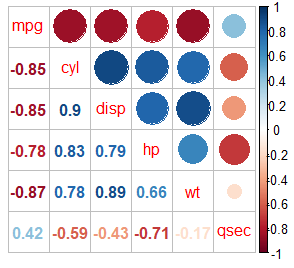
\includegraphics[width=\maxwidth{.95\linewidth}]{gfx/14-corplot}
	\caption{Correlation Plot}
	\label{14:fig04}
\end{figure}

In the correlation plot, the names of the variables are listed diagonally from the top left to the bottom right. In the lower half of the plot the correlations are reported numerically. Thus, the correlation between ``mpg'' and ``cyl'' is $ -0.85 $. Those correlations are also color-coded using the scale found on the right side of the plot. Since $ -0.85 $ is a fairly strong negative correlation it is printed in a dark red color. The top half of the plot shows the correlations using circles where both color and size indicate the strength and direction of the correlation. Thus, the correlation between ``wt'' and ``qsec'' is very weak since the size of the circle is small and it is negative since the color is pale pink. Using a correlation plot, researchers can very quickly locate strong positive and negative correlations, like ``mpg'' and ``wt'' (strong negative) or ``disp'' and ``wt'' (strong positive).

Another useful tool is a scatter plot. Consider Figure \ref{14:fig05}, which shows the relationship between the waiting time and eruption time for the Old Faithful geyser in Yellowstone Park \footnote{These data were first published by H{\"a}rdle in \textit{Smoothing Techniques with Implementation in S}\cite{hardle2012smoothing}.}. The plot clearly shows that the longer people have to wait for an eruption (time along the X-Axis increases) then the longer the eruption will last (time along the Y-Axis increases). This scatter plot also shows two clear groups of points so it would be reasonable to conclude that there are ``short'' eruptions and ``long'' eruptions.

\begin{figure}[H]
	\centering
	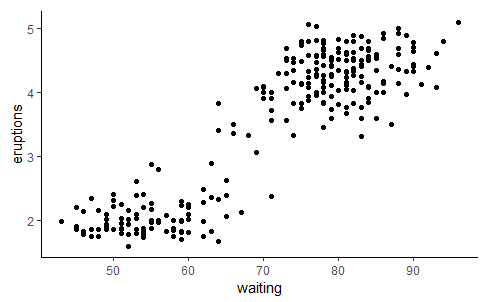
\includegraphics[width=\maxwidth{.95\linewidth}]{gfx/14-Faithful}
	\caption{Scatter Plot}
	\label{14:fig05}
\end{figure}

\subsection{Quantitative Analysis: Inferential}
%TODO Bhattacherjee p 138

Inferential statistics are procedures used to reach conclusions about the associations between variables. They differ from descriptive statistics in that they are explicitly designed to test hypotheses. Numerous statistical procedures fall in this category but all are supported by statistical software like \textit{R}. This chapter provides only a short primer on the most basic and frequent inferential procedures.

\subsubsection{Hypothesis Testing}

A hypothesis is a proposition put forth to explain some observed phenomena. Often, a hypothesis also functions in a predictive manner and is capable of being tested by scientific methods. For example, a researcher might hypothesize the following: Ads placed in a local newspaper are more effective than those placed on a local radio station. This hypothesis could then be tested by placing ads in both media and measuring the results of those ads. Hypothesis typically have these characteristics:

\begin{itemize}
	\item Clear. The hypothesis must be stated in clear and precise language.
	\item Testable. A hypothesis must be testable with some way to determine if the hypothesis is true or false.
	\item Consistent. A hypothesis should be consistent with known facts or an established body of literature.
	\item Timely. A hypothesis must be able to be confirmed (or rejected) in a reasonable time frame.
\end{itemize} 

It is normally not possible to actually prove a hypothesis since it is not possible to have all relevant data to analyze. In the case of the advertising media mentioned above, it would not be possible to prove that hypothesis for every possible combination of newspaper and radio, in all possible markets, in all possible seasons, for all possible products. Thus, researcher projects normally include both a \textit{Null Hypothesis} and an \textit{Alternative Hypothesis}. While these appear to be two different hypothesis, they are actually only two sides of a single hypothesis. The alternative hypothesis attempts to explain some phenomena while the null hypothesis, generally, states that the explanation is wrong. For example, consider this hypothesis and its null:

\begin{description}
	\item[Alternative] Ads placed in a local newspaper are more effective than those placed on a local radio station.
	\item[Null] The type of media does not change the effectiveness of an ad.
\end{description}

Often, the difference between an alternative and null hypothesis is explained in the context of a criminal trial. A defendant is considered ``innocent until proven guilty'' so the prosecutor's alternative hypothesis is ``this person robbed the bank'' while the defense supports the null hypothesis that ``this person did not rob the bank.''

The alternative hypothesis cannot be proven, or even tested, directly. Rather, it is tested indirectly by rejecting the null hypotheses by using a defined level of probability. It is not possible to know with certainty that the conclusion of a research project, which is based on a sample, also applies to the entire population since the sample is never equal to the population. The probability that a conclusion is caused by mere chance is called the \textit{p-value} (for ``probability value''). The \textit{p-value} is the maximum level of acceptable risk that the project's conclusion is \textit{in}correct. For most business and marketing research, in fact, most research in any of the social sciences, a \textit{p-value} of $ 0.05 $ (or $ 5\% $) is considered the cutoff for significance. A calculated \textit{p-value} that is less than $ 0.05 $ indicates that there is enough statistical evidence to reject the null hypothesis, and consequently, accept the alternative hypothesis. If the \textit{p-value} is greater than $ 0.05 $ then the null hypothesis cannot be rejected. All statistics programs, like \textit{R}, calculates a \textit{p-value} as part of the output for many statistical tests so researchers do not have to do anything special to find that value.

\subsubsection{Comparing Two Groups}

One of the simplest inferential analyses is comparing the outcomes of treatment and control groups in a randomized post-test only design. For example, determining whether students enrolled in an ``enhanced'' mathematics program perform better than those in a traditional program. In this case, the variable that predicts the student's performance is a dummy variable, where $ 1 $ is treatment group and $ 0 $ is the control group, and the outcome variable, performance, is a test score following the mathematics courses. The analytic technique for this simple design is a one-way \textit{ANOVA}, or ``Analysis of Variance,'' (one-way because it involves only one predictor variable) and the statistical test used is called a \textit{t-test}.\footnote{The \textit{t-test} was introduced in $ 1908 $ by William Sealy Gosset, a chemist working for the Guiness Brewery in Dublin, Ireland, to monitor the quality of stout --- a dark beer popular with nineteenth-century porters in London. Because his employer did not want to reveal the fact that it was using statistics for quality control, Gosset published the test in \textit{Biometrika} using his pen name ``Student.'' The test involved calculating the value of ``t,'' which was a letter used frequently to denote the difference between two groups. Hence, the name ``Student's t-test.''}

The t-test examines whether the means of two groups are statistically different from each other (non-directional or two-tailed test), or whether one group has a statistically larger (or smaller) mean than the other (directional or one-tailed test). In the mathematics example, if the goal is to examine whether students in the enhanced mathematics program perform better than those in a traditional program it would be a one-tailed test. The hypothesis can be stated as:

\begin{description}
	\item[Alternate] The enhanced program scores are greater than the traditional program scores.
	\item[Null] The enhanced program scores are less than or equal to the traditional program scores.
\end{description}

Note that the null hypothesis always contains an ``equal'' sign and the goal of a statistical significance test is to reject the null hypothesis. Imagine that a random sample of scores is drawn from each of the two groups and the mean of the ``traditional'' group is $ 45 $ while the mean of the ``enhanced'' group is $ 65 $. These two means are certainly different, but that difference may not be significant. For example, the actual scores from the two groups of students may be the same but the random samples happened to be different by chance. A t-test is used to determine if two means actually indicate differences in two populations or if any perceived difference is just chance. The results of a t-test is a \textit{p-value} and if that value is less than $ 0.05 $ then researchers can assume that the means are truly different and then reject the null hypothesis.

Extending from the mathematics program example, imagine that the effect of the enhanced program relative to the traditional program depends on the amount of instructional time is offered, either three or six hours/week. This creates what is called a $ 2 x 2 $ factorial design, with the two factors being program type (enhanced vs. traditional) and instructional time (three vs. six hours/week). This type of design helps researchers estimate the independent effect of each factor, called \textit{main effects}, but also the joint effect of both factors, called the \textit{interaction effect}. This type of factorial design can be analyzed using a two-way \textit{ANOVA} analysis. 

\subsubsection{Other Quantitative Analysis}

There are many other useful inferential statistical techniques that are briefly mentioned here.

\begin{itemize}
	\item Factor analysis is a data reduction technique that is used to statistically aggregate a large number of observed measures (items) into a smaller set of unobserved (latent) variables called factors based on their underlying bi-variate correlation patterns.
	\item Discriminant analysis is a classification technique that aims to place a given observation in one of several nominal categories based on a linear combination of predictor variables. It is popular in marketing applications, such as for classifying customers or products into categories based on salient attributes as identified from large-scale surveys.
	\item Logistic regression is a model in which the outcome variable is binary (zero or one) and is presumed to follow a logistic distribution. The goal of the regression analysis is to predict the probability of the successful outcome by fitting data into a logistic curve. An example is predicting the probability of heart attack within a specific period, based on predictors such as age, body mass index, exercise regimen, and so forth. Logistic regression is extremely popular in the medical sciences. 
	\item Probit regression is a model in which the outcome variable can vary between zero and one and is presumed to follow a standard normal distribution. The goal of the regression is to predict the probability of each outcome. This is a popular technique for predictive analysis in the actuarial science, financial services, insurance, and other industries for applications such as credit scoring based on a person's credit rating, salary, debt and other information from a loan application.
	\item Path analysis is a technique for analyzing directional relationships among a set of variables. It allows for examination of complex models where the dependent variable in one equation is the independent variable in another equation, and is widely used in contemporary social science research. 
	\item Time series analysis is a technique for analyzing time series data, or variables that continually changes with time. Examples of applications include forecasting stock market fluctuations and urban crime rates. This technique is popular in econometrics, mathematical finance, and signal processing. Special techniques are used to correct for auto-correlation, or correlation within values of the same variable across time 
\end{itemize}

\section{Qualitative Analysis}
%TODO Bhattacherjee p 122

Qualitative analysis is the analysis of qualitative data such as text data from interview transcripts. Unlike quantitative analysis, which is statistics driven and largely independent of the researcher, qualitative analysis is heavily dependent on the researcher's analytic and integrative skills and personal knowledge of the social context where the data is collected. The emphasis in qualitative analysis is ``sense making'' or understanding a phenomenon rather than predicting or explaining. A creative and investigative mindset is needed for qualitative analysis, based on an ethically enlightened and participant-in-context attitude, and a set of analytic strategies. 

\subsection{Grounded Theory}

How is a vast set qualitative data acquired through participant observation, in-depth interviews, focus groups, narratives of audio/video recordings, or secondary documents analyzed? One of these techniques used is \textit{grounded theory} --- an inductive technique of interpreting recorded data about a social phenomenon to build theories about that phenomenon. The technique was developed by Glaser and Strauss\cite{glaser1967discovery} in their method of constant comparative analysis of grounded theory research, and further refined by Corbin and Strauss\cite{corbin1990grounded} to further illustrate specific coding techniques --- a process of classifying and categorizing text data segments into a set of codes (concepts), categories (constructs), and relationships. The interpretations are ``grounded in'' (or based on) observed empirical data, hence the name. To ensure that the theory is based solely on observed evidence, the grounded theory approach requires that researchers suspend any preexisting theoretical expectations or biases before data analysis and let the data dictate the formulation of the theory.

Strauss and Corbin\cite{strauss1998basics} describe three coding techniques for analyzing text data: open, axial, and selective. 

Open coding is a process aimed at identifying concepts or key ideas that are hidden within textual data, which are potentially related to the phenomenon of interest. The researcher examines the raw textual data line by line to identify discrete events, incidents, ideas, actions, perceptions, and interactions of relevance that are coded as concepts (hence called in vivo codes). Each concept is linked to specific portions of the text (coding unit) for later validation. Some concepts may be simple, clear, and unambiguous while others may be complex, ambiguous, and viewed differently by different participants. The coding unit may vary with the concepts being extracted. Simple concepts such as ``organizational size'' may include just a few words of text, while complex ones such as ``organizational mission'' may span several pages. Concepts can be named using the researcher’s own naming convention or standardized labels taken from the research literature. Once a basic set of concepts are identified, these concepts can then be used to code the remainder of the data, while simultaneously looking for new concepts and refining old concepts. While coding, it is important to identify the recognizable characteristics of each concept, such as its size, color, or level (e.g., high or low), so that similar concepts can be grouped together later. This coding technique is called ``open'' because the researcher is open to and actively seeking new concepts relevant to the phenomenon of interest.

Axial coding groups codes into higher order categories. While concepts may be context-specific, categories tend to be broad and generalizable, and ultimately evolve into constructs in a grounded theory. Categories are needed to reduce the amount of concepts the researcher must work with and to build a ``big picture'' of the issues salient to understanding a social phenomenon. Categorization can be done is phases, by combining concepts into subcategories, and then subcategories into higher order categories. Constructs from the existing literature can be used to name these categories, particularly if the goal of the research is to extend current theories. However, caution must be taken while using existing constructs, as such constructs may bring with them commonly held beliefs and biases. For each category, its characteristics (or properties) and dimensions of each characteristic should be identified. The dimension represents a value of a characteristic along a continuum. For example, a ``communication media'' category may have a characteristic called ``speed,'' which can be dimensionalized as fast, medium, or slow. Such categorization helps differentiate between different kinds of communication media and enables researchers identify patterns in the data, such as which communication media is used for which types of tasks. The second phase of grounded theory is axial coding, where the categories and subcategories are assembled into causal relationships or hypotheses that can tentatively explain the phenomenon of interest. Although distinct from open coding, axial coding can be performed simultaneously with open coding. The relationships between categories may be clearly evident in the data or may be more subtle and implicit. In the latter instance, researchers may use a coding scheme to understand which categories represent conditions (the circumstances in which the phenomenon is embedded), actions/interactions (the responses of individuals to events under these conditions), and consequences (the outcomes of actions/ interactions). As conditions, actions/interactions, and consequences are identified, theoretical propositions start to emerge, and researchers can start explaining why a phenomenon occurs, under what conditions, and with what consequences.

The third and final phase of grounded theory is selective coding, which involves identifying a central category or a core variable and systematically and logically relating this central category to other categories. The central category can evolve from existing categories or can be a higher order category that subsumes previously coded categories. New data is selectively sampled to validate the central category and its relationships to other categories (i.e., the tentative theory). Selective coding limits the range of analysis, and makes it move fast. 

At the same time, the coder must watch out for other categories that may emerge from the new data that may be related to the phenomenon of interest (open coding), which may lead to further refinement of the initial theory. Hence, open, axial, and selective coding may proceed simultaneously. Coding of new data and theory refinement continues until theoretical saturation is reached, i.e., when additional data does not yield any marginal change in the core categories or the relationships.

The ``constant comparison'' process implies continuous rearrangement, aggregation, and refinement of categories, relationships, and interpretations based on increasing depth of understanding, and an iterative interplay of four stages of activities: (1) comparing incidents/texts assigned to each category (to validate the category), (2) integrating categories and their properties, (3) delimiting the theory (focusing on the core concepts and ignoring less relevant concepts), and (4) writing theory. Having a central category does not necessarily mean that all other categories can be integrated nicely around it. In order to identify key categories that are conditions, action/interactions, and consequences of the core category techniques such as storylining, memoing, or concept mapping are used. In storylining, categories and relationships are used to explicate and/or refine a story of the observed phenomenon. Memos are theorized write-ups of ideas about substantive concepts and their theoretically coded relationships as they evolve during ground theory analysis, and are important tools to keep track of and refine ideas that develop during the analysis. Memoing is the process of using these memos to discover patterns and relationships between categories using two-by-two tables, diagrams, or figures, or other illustrative displays. Concept mapping is a graphical representation of concepts and relationships between those concepts (e.g., using boxes and arrows). The major concepts are typically laid out on one or more sheets of paper, blackboards, or using graphical software programs, linked to each other using arrows, and readjusted to best fit the observed data.

After a grounded theory is generated, it must be refined for internal consistency and logic. Researchers must ensure that the central construct has the stated characteristics and dimensions, and if not, the data analysis may be repeated. Researcher must then ensure that the characteristics and dimensions of all categories show variation. For example, if behavior frequency is one such category, then the data must provide evidence of both frequent performers and infrequent performers of the focal behavior. Finally, the theory must be validated by comparing it with raw data. If the theory contradicts with observed evidence, the coding process may be repeated to reconcile such contradictions or unexplained variations. 

\section{Quantitative vs. Qualitative}

Given their differences, it may come as no surprise that quantitative and qualitative research in psychology and related fields do not coexist in complete harmony. Some quantitative researchers criticize qualitative methods on the grounds that they lack objectivity, are difficult to evaluate in terms of reliability and validity, and do not allow generalization to people or situations other than those actually studied. At the same time, some qualitative researchers criticize quantitative methods on the grounds that they overlook the richness of human behavior and experience and instead answer simple questions about easily quantifiable variables.

In general, however, qualitative researchers are well aware of the issues of objectivity, reliability, validity, and generalizability. In fact, they have developed a number of frameworks for addressing these issues (which are beyond the scope of our discussion). And in general, quantitative researchers are well aware of the issue of oversimplification. They do not believe that all human behavior and experience can be adequately described in terms of a small number of variables and the statistical relationships among them. Instead, they use simplification as a strategy for uncovering general principles of human behavior.

\section{Combining Quantitative and Qualitative}

Quantitative research (i.e., a positivist paradigm) has historically been the cornerstone of business and marketing research. Purists call for researchers to ``eliminate their biases, remain emotionally detached and uninvolved with the objects of study and test or empirically justify their stated hypotheses''\cite{johnson2004mixed}.

Qualitative purists support a constructivist or interpretivist paradigm and ``contend that multiple-constructed realities abound, that time- and context free generalizations are neither desirable nor possible, that research is value-bound, that it is impossible to differentiate fully causes and effects, that logic flows from specific to general and that knower and known cannot be separated because the subjective knower is the only source of reality''\cite{johnson2004mixed}.

It was in the 80's and 90's that researchers began to call for a ``truce'' in the ``Paradigm Wars'' between quantitative and qualitative methods. Many major authors and researchers felt that the two research methodologies are compatible and could be combined in a single research project. In fact, the proverbial pendulum has swung the other direction and many researchers now believe that there is no major problem area that should be studied exclusively with one research method. They believe that quantitative research answers the ``if'' question while qualitative research answers the ``how or why.'' This research paradigm is known as a ``mixed-methods'' approach, though other phrases are occasionally used, like multi-modal.

%TODO from Lorenzini
Mixed-method research offers powerful tools to investigate complex systems and processes in business, marketing, and economics. This method includes all phases of a research project, including philosophical assumptions, research questions, design, collection, analysis, integration and presentation of data and results. \footnote{The material in this section is adapted from Lorenzini, \textit{Mixed-Method Research in the Health Sciences}\cite{lorenzini2017mixed}}

The nature of the research question guides the selection of the method. Researchers in business-related fields use a quantitative methodology to study and answer research questions on causality, generalization, and magnitude of effect. The qualitative methodology is the choice of researchers who seek to answer research questions that explore how or why a given phenomenon occurs, to develop a theory or describe on the subjectivity of an individual experience.

Mixed-method research attempts to utilize the strengths of each of the two approaches, quantitative and qualitative, and, for this reason, it is being increasingly used to address contemporary research problems. An indication of the increased interest of this method was the publication of guidelines on mixed-methods research in various fields, like information systems\cite{venkatesh2013bridging} and health sciences\cite{creswell2004designing}.

Over the course of the years, several definitions of mixed methods have emerged incorporating characteristics of method, philosophy, processes, and research projects. Researchers, though, seem to be focused on defining mixed-methods by its characteristics, which are described:

\begin{itemize}
	\item the collection and analysis of both quantitative and qualitative data takes place;

	\item rigorous procedures are used to carry out quantitative and qualitative research;

	\item there is integration or combination of results;

	\item procedures are developed in which data collection, analysis, and integration takes place, in other words, a mixed-methods design;
\end{itemize}

It is, therefore, pointed out that this method involves the triangulation of quantitative and qualitative data in a single project. Those approaches complement each other inasmuch as they represent words and numbers, the two fundamental languages of human communication. Among the advantages of mixed methods, it may be stated that researchers can permit the manifestation of the best of each of the methods, avoiding the possible limitations of a single approach. This methodological orientation is indicated when a data source may be insufficient to answer the research problem or when the results need to be explained and the exploratory findings need generalization.

It is often argued that the quantitative approach is not able to capture the specificities in terms of what is understood of the context where the study took place. Still, researchers in this line are at the vanguard and possible or eventual subjective interpretations are rarely discussed. Qualitative research compensates for these weaknesses. However, qualitative research is seen as deficient due to the personal interpretations made by the researcher, the bias created because of this, the small number of participants, and the difficulty to generalize the results. Quantitative research, in turn, does not have those weaknesses. Thus, the combination of potentialities of one approach compensates for the weaknesses of the other. Thereby, the mixed-methods research provides more evidence for the study of a research problem than the use of one of the two approaches in an isolated manner. By using mixed methods, researchers can use all available tools, rather  than confining themselves to data collection strategies commonly associated with either quantitative or qualitative research. 

Researchers who master one of the approaches and who come from different epistemological perspectives often find themselves working together on a team to that is conducting mixed-methods research. To improve the dynamics of these teams, it is necessary for their members to develop the capacity to articulate their own research philosophy, visions, values, and objectives. Still, it is important to facilitate group interactions by creating conditions for values to be shared through dialogue, defining objectives, and developing trust. Systematically, it is quite important to optimize the values that promote and support dialectic pluralism and participation from stakeholders in research.

The application of integration principles and practices may help researchers to leverage the strong points of mixed methods. Recommendations about the best practices for mixed-methods include the following.

\begin{itemize}
	\item Identify the quantitative and qualitative results;
	\item Be consistent with the design used in the method;
	\item Be consistent with the integration methodology;
	\item Identify inferences, meta-inferences, and insights generated.
\end{itemize}

%TODO This comes from Terrell - Mixed Methods...

\subsection{Strategies}

Mixed-methods projects typically fall into one of three general strategies, listed below and more fully described later in this chapter.

\begin{itemize}
	\item Sequential Explanatory
	\item Sequential Exploratory
	\item Convergent Parallel (Triangulation)
\end{itemize}

The specific type of strategy used depends upon four factors:

\begin{itemize}
	\item Theoretical perspective of the researcher
	\begin{itemize}
		\item Explicit – Does the researcher base the research project directly on a theory?
		\item Implicit – Does the researcher only indirectly use theory as a foundation for the research project?
	\end{itemize}

	\item Priority of strategy
	\begin{itemize}
		\item Qualitative - Is the qualitative portion of the research project more important?
		\item Quantitative - Is the quantitative portion of the research project more important?
		\item Equal - Are the two types of research, quantitative/qualitative, equally used in the research project?
	\end{itemize}

	\item Sequence of data collection implementation
	\begin{itemize}
		\item Is the qualitative part completed first and then the quantitative part done?
		\item Is the quantitative part completed first and then the qualitative part done?
		\item Are both parts completed simultaneously?
	\end{itemize}

	\item The point at which the data are integrated
	\begin{itemize}
		\item At data collection
		\item At data analysis
		\item At data interpretation
		\item With some combination
	\end{itemize}
\end{itemize}

\subsubsection{Sequential Explanatory Strategy}

The sequential explanatory strategy is used when a researcher already has a theory to explain some phenomena and wants to collect data to explain certain facets of that theory. Figure \ref{14:fig90} illustrates the process of a sequential explanatory strategy. 

\begin{figure}[H]
	\centering
	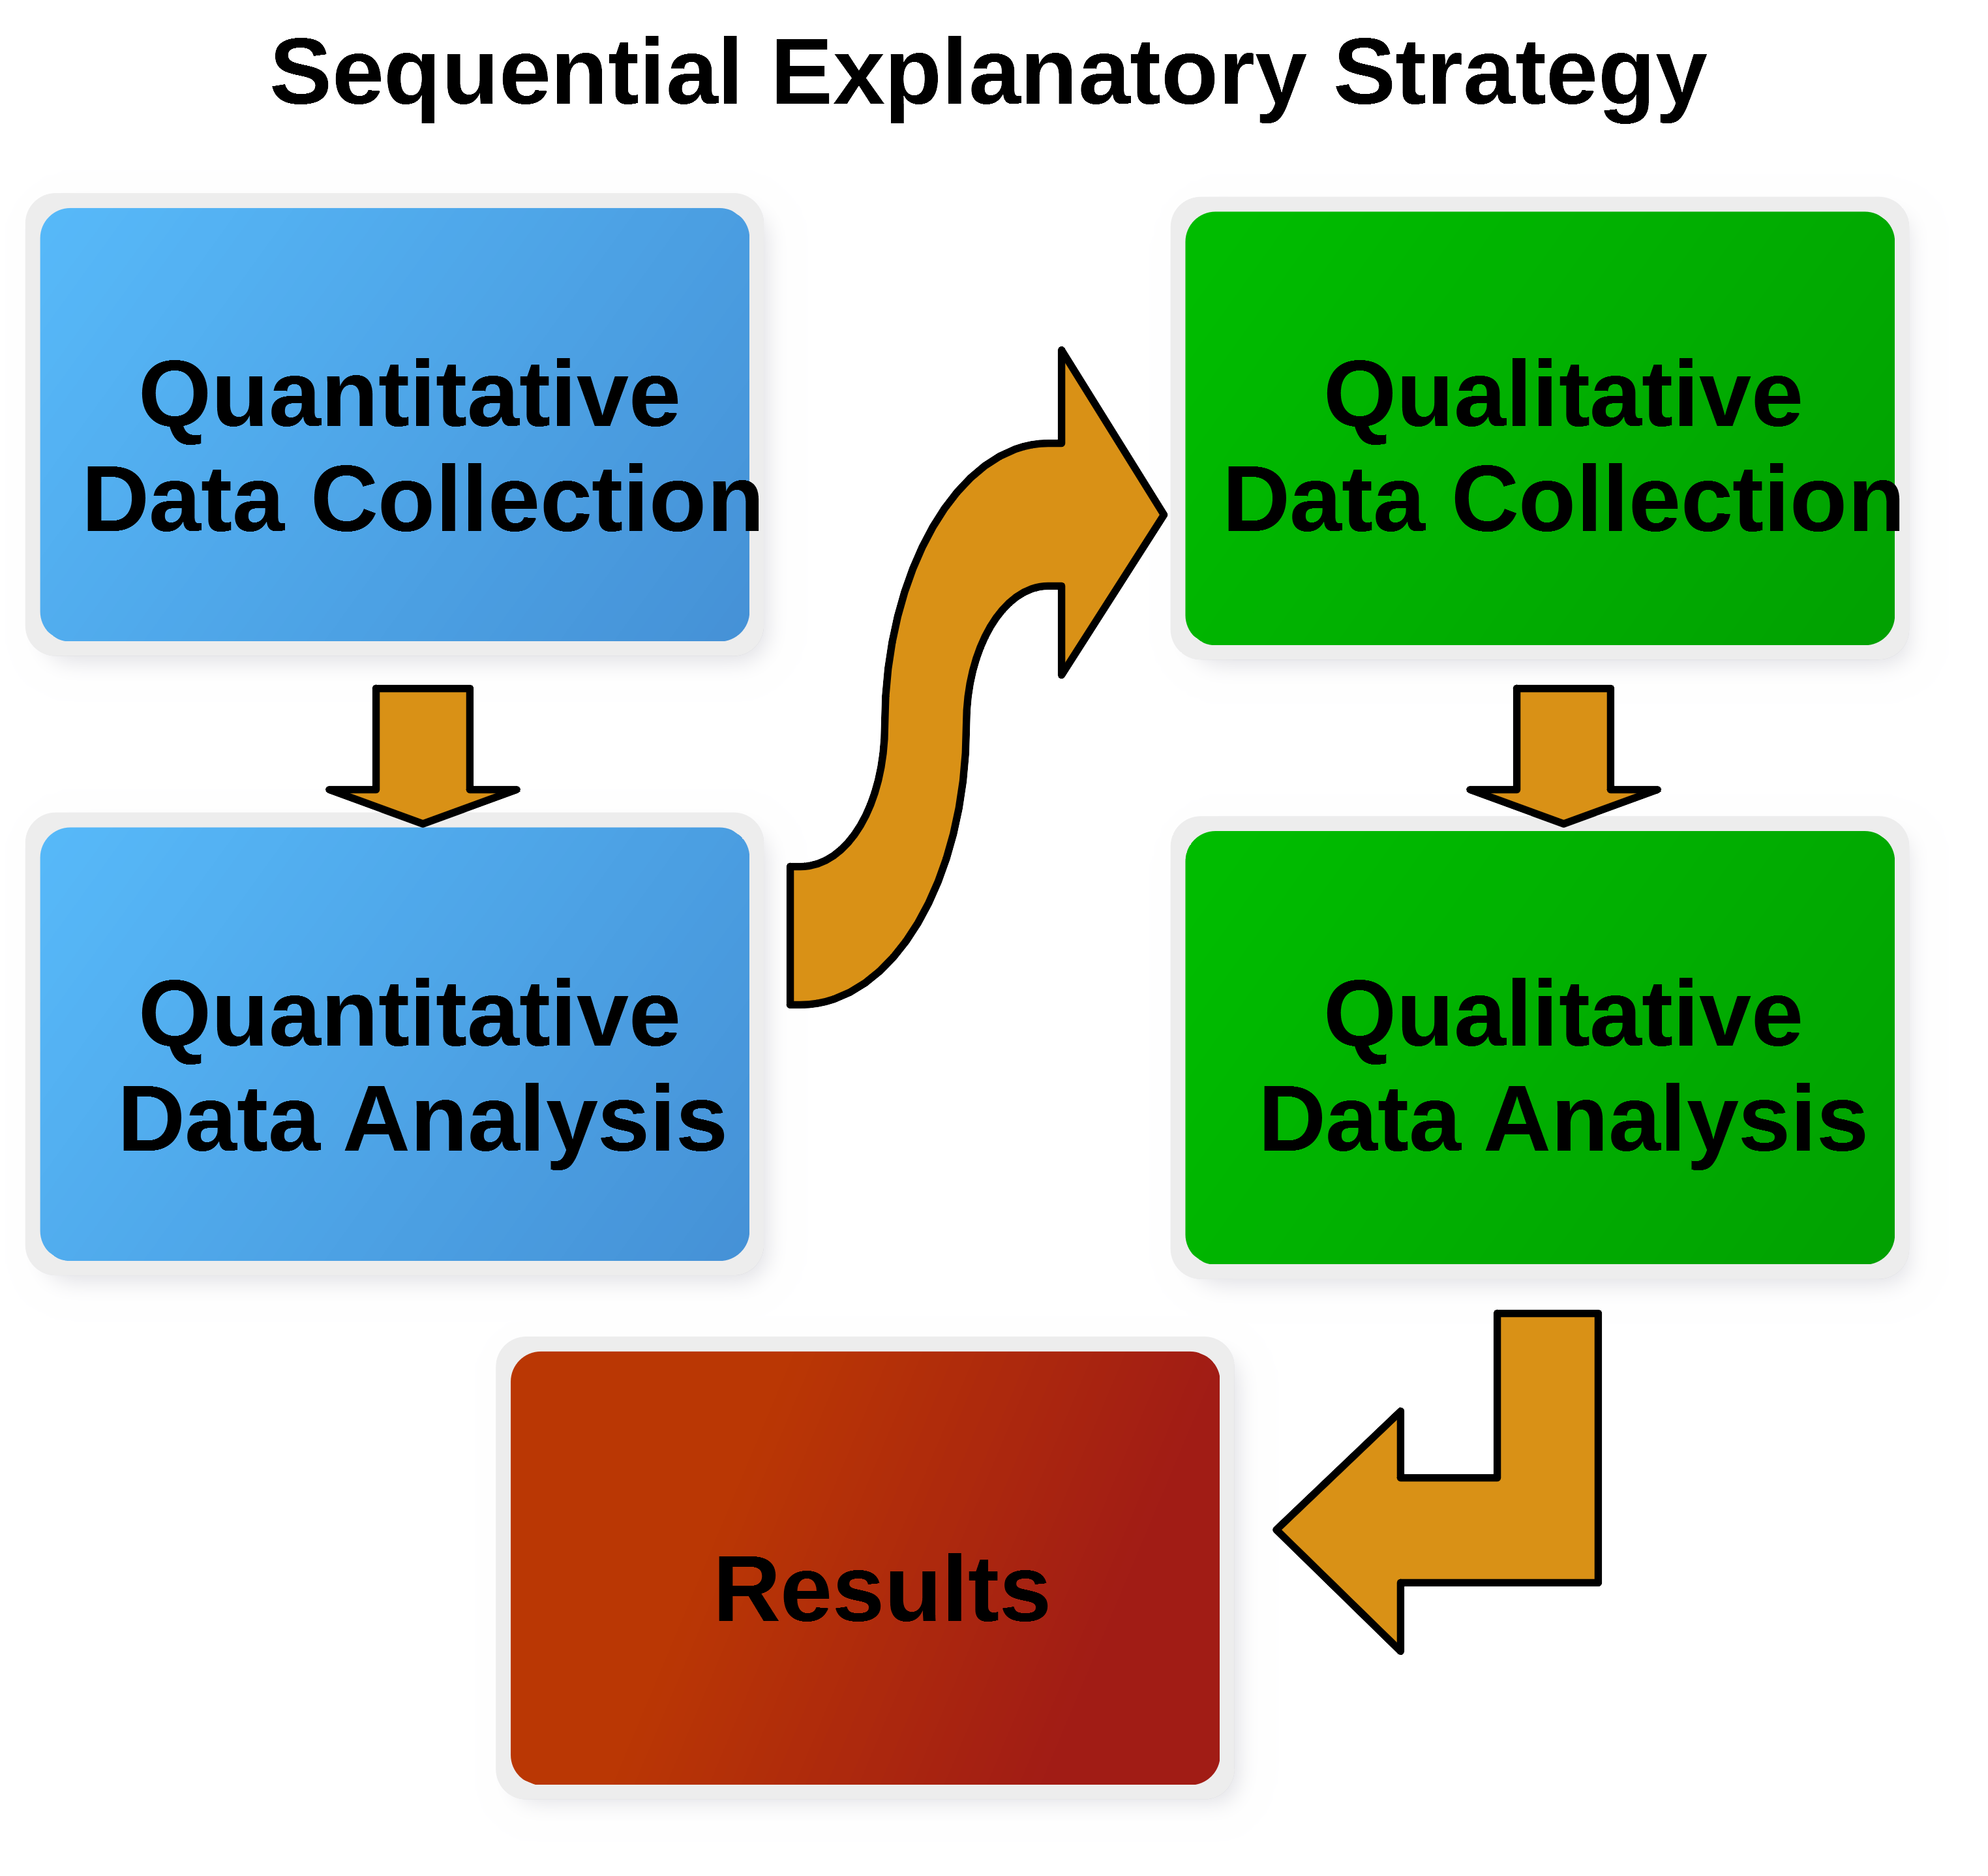
\includegraphics[width=\maxwidth{.95\linewidth}]{gfx/14-Seq_Explain}
	\caption{Sequential Explanatory}
	\label{14:fig90}
\end{figure}

The collection and analysis of quantitative data is followed by the collection and analysis of qualitative data where equal priority is given to the two phases. The data are integrated in the interpretive phase. The primary focus of this strategy is to explain quantitative results by exploring those results in more detail or to help explain unexpected results (e.g., using follow-up interviews to better understand the results of a quantitative study).

\begin{description}
	\item[Strength] --- relatively straight forward due to clear, distinct stages and easier to describe than concurrent strategies.

	\item[Weakness] --- very time consuming especially when both phases are given equal consideration and priority.
\end{description}

\subsubsection{Sequential Exploratory Strategy}

The sequential exploratory strategy is used when a researcher is seeking to develop a theory related to some observation. Figure \ref{14:fig91} illustrates the process of a sequential exploratory strategy. 

\begin{figure}[H]
	\centering
	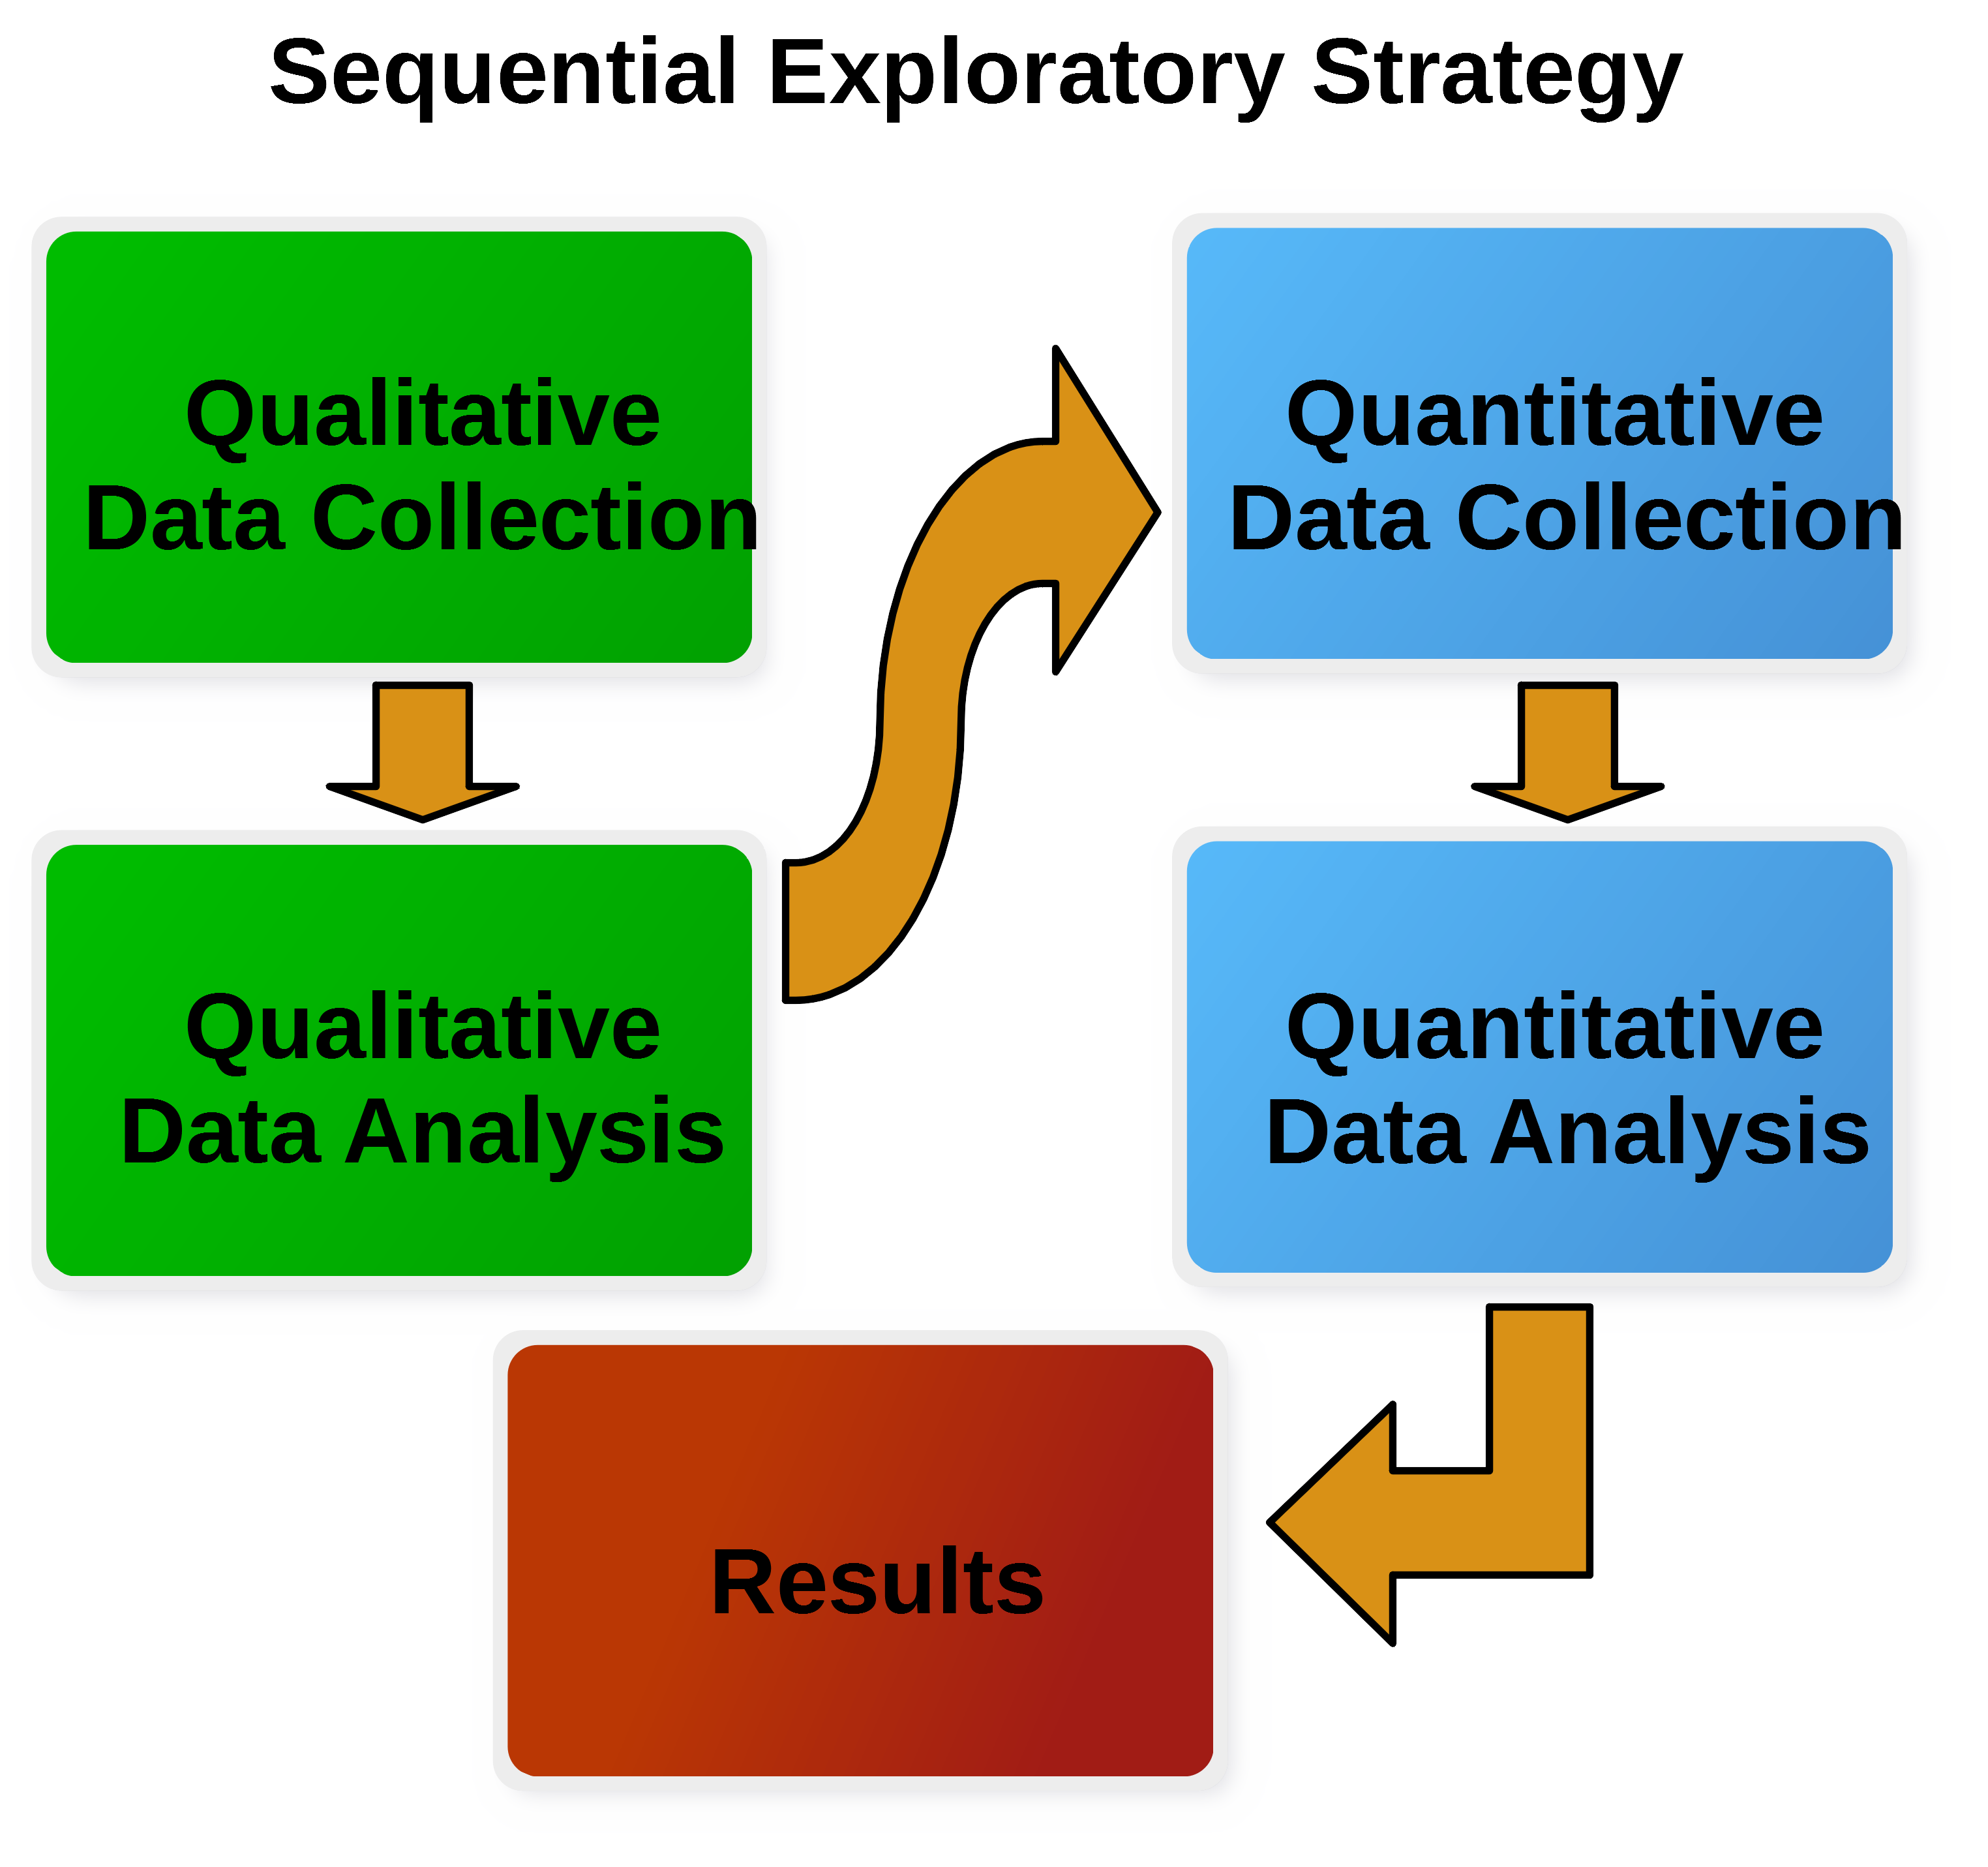
\includegraphics[width=\maxwidth{.95\linewidth}]{gfx/14-Seq_Explore}
	\caption{Sequential Exploratory}
	\label{14:fig91}
\end{figure}

The collection and analysis of qualitative data is followed by the collection and analysis of quantitative data where equal priority is given to the two phases but priority can be given to either as the project unfolds. Data are integrated during interpretation phase. This strategy is used primarily to explore a phenomenon by testing the elements of a theory, generalizing qualitative findings to different samples, and the development of instrumentation (e.g., using a small group to create some sort of instrument, like a survey, and then collecting quantitative data based on that instrument).

\begin{description}
	\item[Strength] --- relatively straight forward due to clear, distinct stages and easier to describe than concurrent strategies.
	\item[Weakness] --- very time consuming, especially when both phases are given equal consideration and priority.
\end{description}

\subsubsection{Convergent Parallel (Triangulation)}

The convergent parallel strategy, often called ``triangulation,'' is used when a researcher is seeking to validate a research project by converging two, or more, research processes on a single observation. Figure \ref{14:fig92} illustrates the process of a convergent parallel strategy. 

\begin{figure}[H]
	\centering
	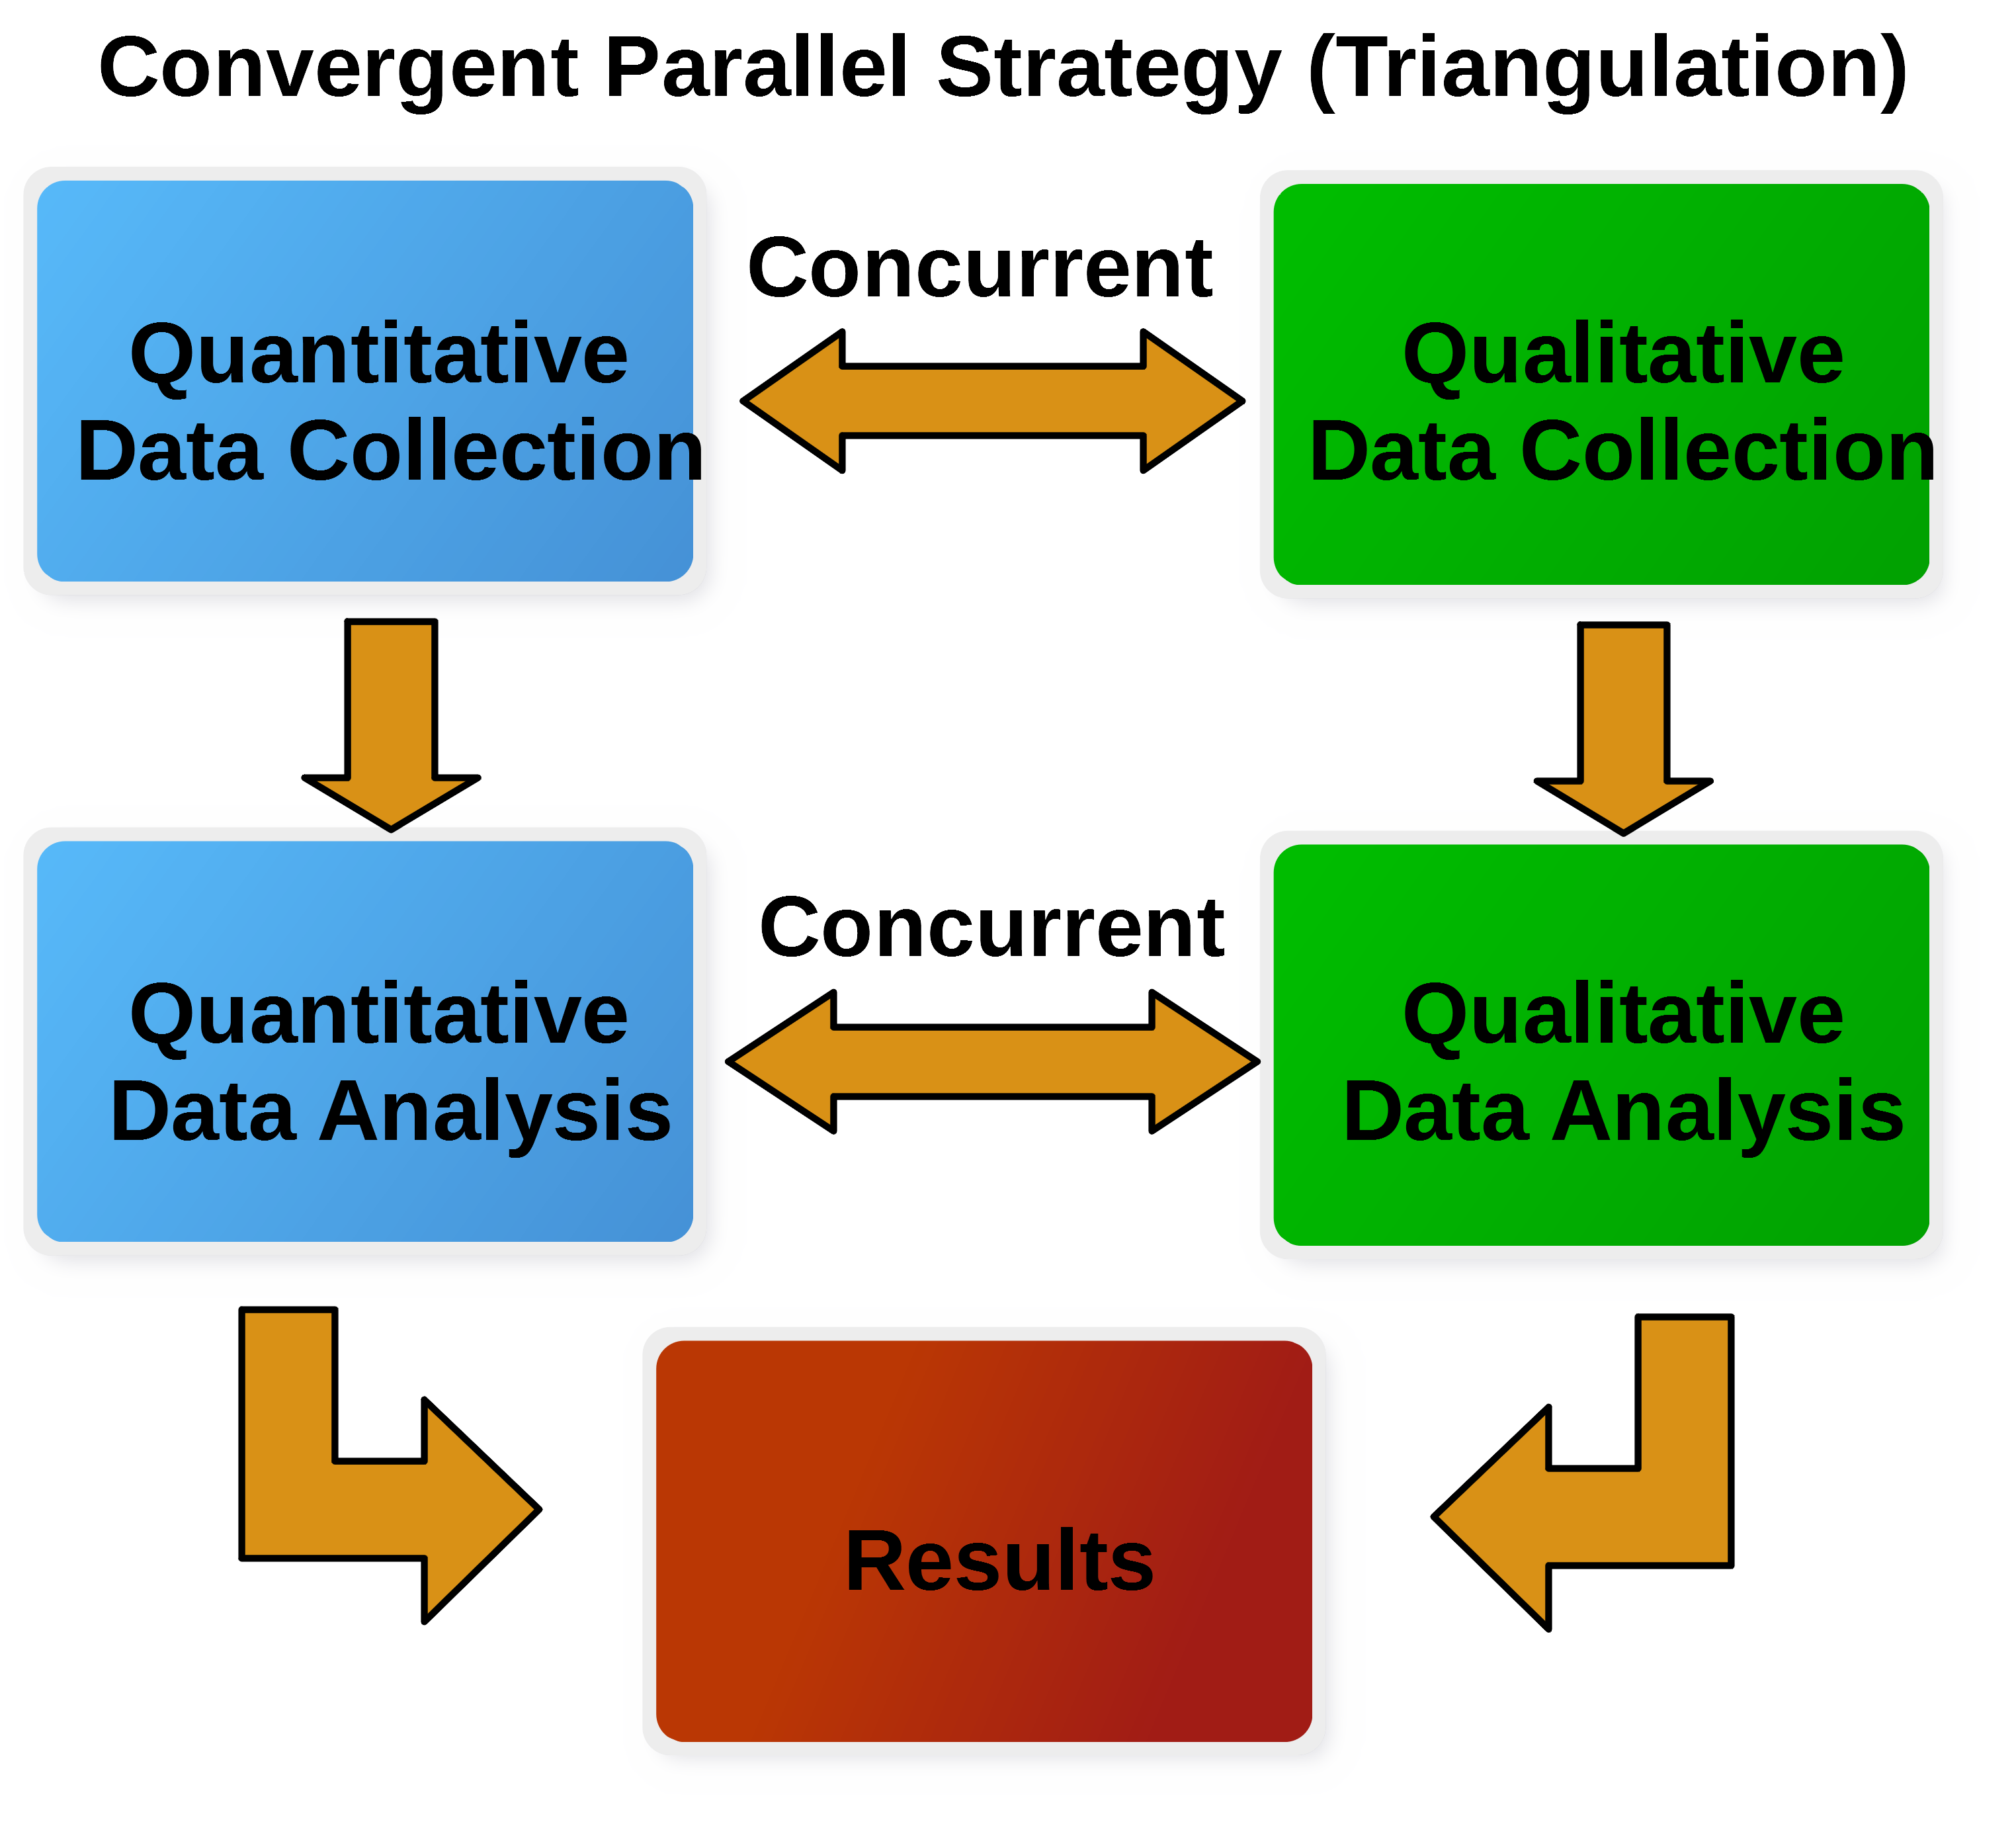
\includegraphics[width=\maxwidth{.95\linewidth}]{gfx/14-Triangulation}
	\caption{Triangulation}
	\label{14:fig92}
\end{figure}

There are two concurrent data collection phases where priority should be equal but can be given to either approach. Data are integrated during interpretation phase. The interpretation notes any sort of convergence that strengthens knowledge claims, or, conversely, a lack of convergence that would tend to disprove the knowledge claims. Data integration can also occur during analysis. It is primarily used for confirmation, corroboration or cross-validation within a single study.

\begin{description}
	\item[Strength] --- familiar to many researchers. Shorter data collection time when compared to sequential methods. Offsets weaknesses inherent to one design by using both.
	\item[Weakness] --- requires a great deal of expertise and effort to study the phenomenon under consideration using two different methods. It may be difficult to compare two types of data as well as resolve discrepancies if they arise.
\end{description}


\section{Summary}\label{ch14:summary}

Lorem ipsum dolor sit amet, consectetuer adipiscing elit. Aenean commodo ligula eget dolor. Aenean massa. Cum sociis natoque penatibus et
